\documentclass{article}
\usepackage{graphicx}
\usepackage{geometry}
\geometry{margin=1in}

\title{Report on Faast-A-Faas-Framework}
\author{Claude}
\date{}

\begin{document}
\maketitle

\section{Introduction}
Faast-A-Faas-Framework is a project that aims to test various cluster configurations for Function as a Service (FaaS) platforms and perform analysis using metrics such as latency, throughput, and resource utilization. This report provides a detailed overview of the project, including the cluster configurations, metrics used, workloads for testing, requirements, and instructions for setting up and running the experiments.

\section{Cluster Configurations}
The project considers the following cluster configurations:

\subsection{Single Pod Cluster}
This configuration contains a single pod with a single container deployed in a single node cluster. The following image illustrates the cluster configuration:

\begin{figure}[H]
   \centering
   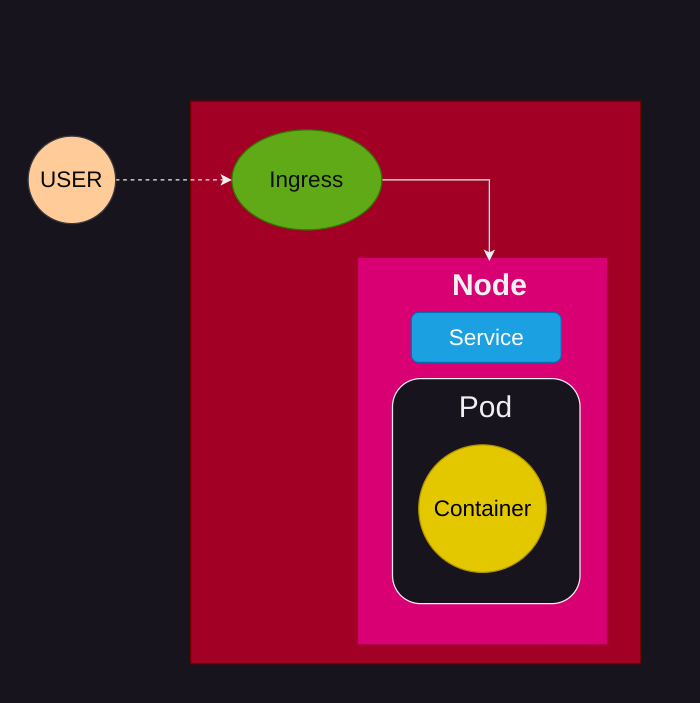
\includegraphics[width=0.5\textwidth]{../images/single_pod.png}
   \caption{Single Pod Cluster}
\end{figure}

\subsection{Single Pod with Multi-Container}
This configuration contains a pod with multiple containers deployed in a single node cluster, with each container running the same service. It also includes a pod that runs an nginx-loadbalancer to route incoming requests to both containers of the pod running the FaaS service. The following image illustrates the cluster configuration:

\begin{figure}[H]
   \centering
   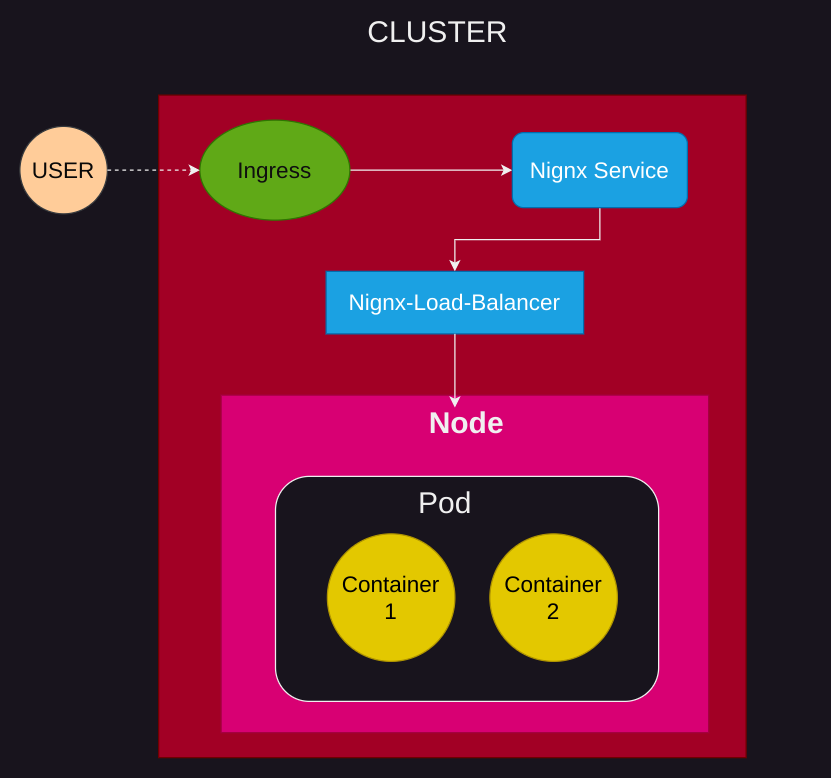
\includegraphics[width=0.5\textwidth]{../images/one_pod_two_container.png}
   \caption{Single Pod with Multi-Container}
\end{figure}

\subsection{Multi-Pod with Single Node}
This configuration contains multiple pods, each containing one container that runs the FaaS service, deployed in a single node. It also includes a pod that runs an nginx-loadbalancer to route incoming requests to the pods running the FaaS service. The following image illustrates the cluster configuration:

\begin{figure}[H]
   \centering
   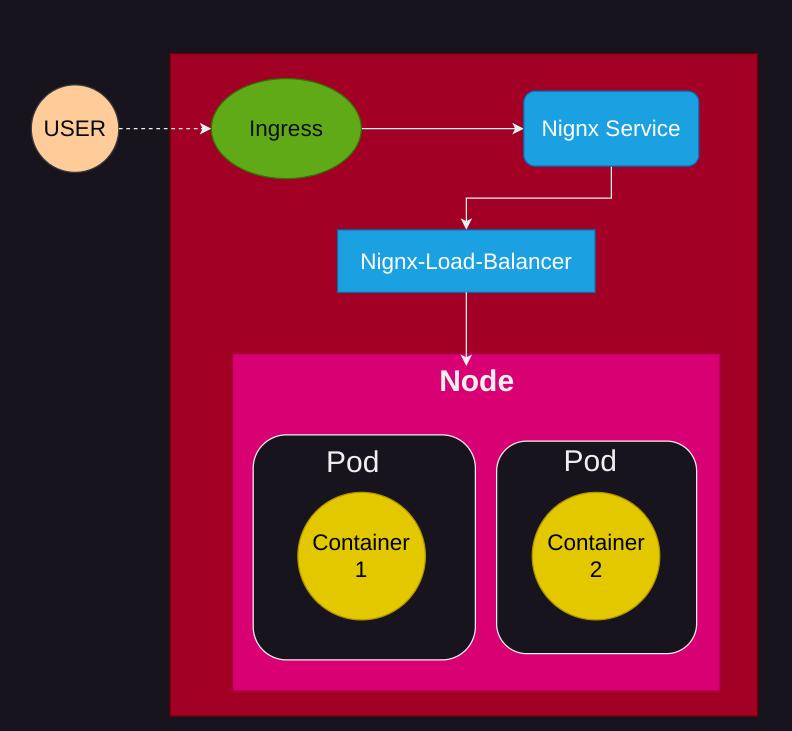
\includegraphics[width=0.5\textwidth]{../images/one_node_two_pod.png}
   \caption{Multi-Pod with Single Node}
\end{figure}

\subsection{Multi-Pod with Multi-Node}
This configuration contains multiple pods, each containing one container that runs the FaaS service, deployed in two different nodes. It also includes a pod that runs an nginx-loadbalancer to route incoming requests to the pods running the FaaS service via their respective services. The following image illustrates the cluster configuration:

\begin{figure}[H]
   \centering
   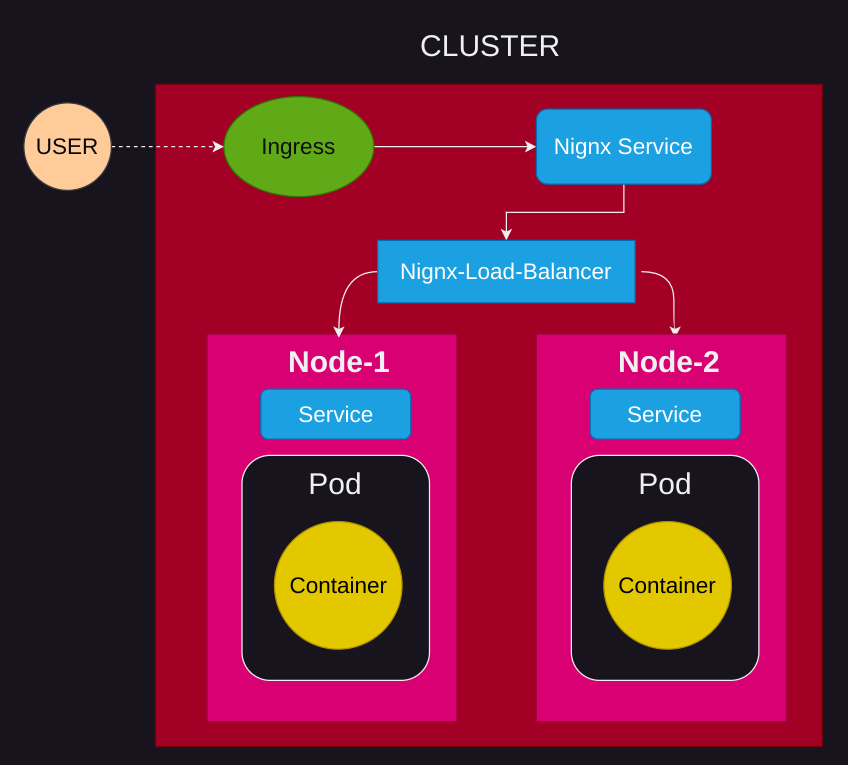
\includegraphics[width=0.5\textwidth]{../images/two_node.png}
   \caption{Multi-Pod with Multi-Node}
\end{figure}

\subsection{Horizontal Pod Autoscaler}
This configuration contains multiple replica sets of pods (initially containing a single pod) deployed in a single node. The Horizontal Pod Autoscaler (HPA) scales out when the resource requirements go beyond the set limits and adjusts the number of pods accordingly. The following image illustrates the cluster configuration:

\begin{figure}[H]
   \centering
   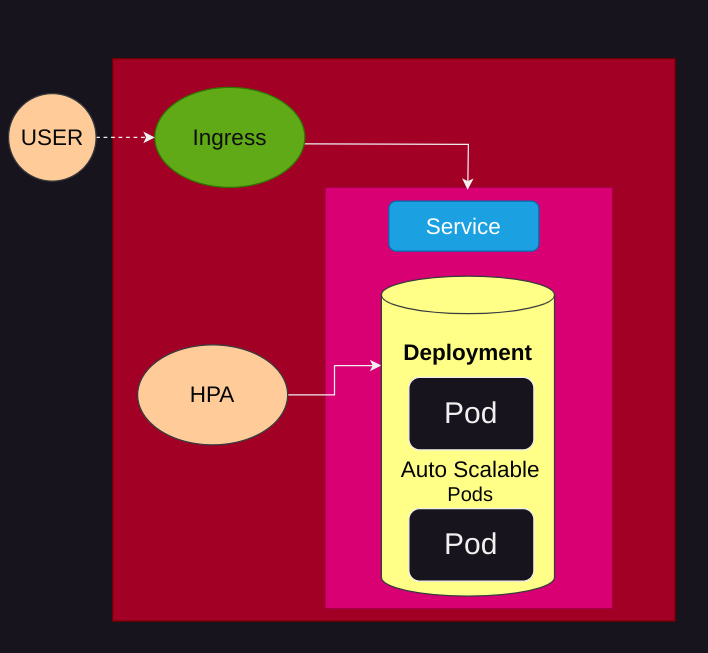
\includegraphics[width=0.5\textwidth]{../images/hpa.png}
   \caption{Horizontal Pod Autoscaler}
\end{figure}

\subsection{Vertical Pod Autoscaler}
This configuration contains a single pod enabled with Vertical Pod Autoscaler (VPA) deployed in a single node. The VPA scales up when the resource requirements go beyond the set limits and adjusts the pod resources accordingly. The following image illustrates the cluster configuration:

\begin{figure}[H]
   \centering
   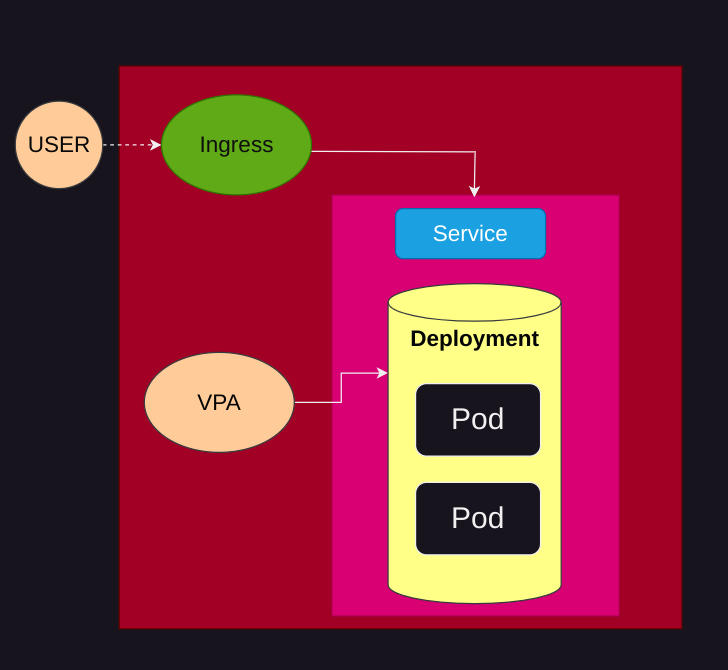
\includegraphics[width=0.5\textwidth]{../images/vpa.png}
   \caption{Vertical Pod Autoscaler}
\end{figure}

\section{Metrics}
The project measures the following metrics:

\subsection{Latency and Throughput}
The latency and throughput of the FaaS service are measured using the `wrk` tool. The analysis is performed for different cluster configurations, and the results are compared. The following image shows the latency and throughput comparison for different cluster configurations:

\begin{figure}[H]
   \centering
   %\includegraphics[width=0.8\textwidth]{latency_throughput.png}
   \caption{Latency and Throughput Comparison}
\end{figure}

\subsection{Resource Utilization (CPU + Mem)}
The CPU and memory utilization of the FaaS service are measured using the `metrics-server` API of Kubernetes. The analysis is performed for different cluster configurations, and the results are compared.

\section{Workloads for Testing}
The project uses two types of simple stateless workloads to test various cluster environments:

\subsection{Beautiful Loops}
This workload runs a for loop performing some simple computations.

\subsection{Random Weird Text}
This workload generates some random text and returns it as a response.

\section{Requirements}
To run the experiments, the following tools need to be installed:

\begin{itemize}
   \item docker
   \item kubectl
   \item minikube
   \item helm
\end{itemize}

\section{Running Instructions for Setting up a Cluster Environment}
To set up the environment for running cluster configurations, run the following command:

\begin{verbatim}
bash setup.sh
\end{verbatim}

The supported app-types based on the cluster configurations defined above are:

\begin{verbatim}
single-pod  two-pod-same-node  two-pod-diff-node  hpa  vpa  two-container
\end{verbatim}

To set up the requirements for running clusters, run the following command with the appropriate `<app_type>`:

\begin{verbatim}
bash deploy_app.sh <app_name> <app_type> <docker_image_name> <python-app-file> <requirements-file> <port> <map_url>
\end{verbatim}

\section{Generating Analysis Results}
To generate analysis results, follow these steps:

\begin{enumerate}
   \item Set up the `metrics-server` REST-API by running the following command in two different terminal windows:
   
   \begin{verbatim}
   minikube dashboard --port=20000
   \end{verbatim}
   
   \item Run the following command to perform the analysis for different cluster configurations and generate logs for response-time and resource utilization:
   
   \begin{verbatim}
   bash src/analysis/perform_analysis.sh <host> <url> <app-type> <app-name>
   \end{verbatim}
   
   This will generate logs for response-time and resource utilization based on the defined workload. The file names will be in the following format:
   
   \begin{verbatim}
   <logs-dir>/<app-name>-<app-type>-response_time.csv
   <logs-dir>/<app-name>-<app-type>-resource_usage.csv
   \end{verbatim}
   
   \item Execute the following Python file to generate plots for the analysis:
   
   \begin{verbatim}
   python3 analysis/get_plot_from_log.py
   usage: script to generate plot from log files [-h] --app-type APP_TYPE
                                                 [--response-log RESPONSE_LOG]
                                                 [--resources-log RESOURCES_LOG] --output-folder
                                                 OUTPUT_FOLDER --app-name APP_NAME

   options:
     -h, --help            show this help message and exit
     --app-type APP_TYPE   single-pod/two-pod-same-node/two-pod-diff-node/hpa/vpa/two-container
     --response-log RESPONSE_LOG
     --resources-log RESOURCES_LOG
     --output-folder OUTPUT_FOLDER
     --app-name APP_NAME
   \end{verbatim}
\end{enumerate}

\end{document}
